\documentclass{article}

\usepackage[utf8]{inputenc}
\usepackage[T1]{fontenc}
\usepackage{fancyhdr}
\usepackage{geometry}
\usepackage{array}
\usepackage[usenames,dvipsnames,svgnames,table]{xcolor}
\usepackage{multirow}
\usepackage{morefloats}
\usepackage{float}
\usepackage{soul}
\usepackage{color}
\usepackage{seqsplit}
\usepackage{gensymb}
\usepackage{siunitx}
\usepackage{graphicx}
\usepackage{pdfpages}
\usepackage[framemethod=TikZ]{mdframed}
\setcounter{secnumdepth}{3}

\usepackage[procnames]{listings}
\usepackage{color}

\definecolor{keywords}{RGB}{255,0,90}
\definecolor{comments}{RGB}{0,0,113}
\definecolor{red}{RGB}{160,0,0}
\definecolor{green}{RGB}{0,150,0}

\lstset{language=Python,
        basicstyle=\ttfamily\small,
        keywordstyle=\color{keywords},
        commentstyle=\color{comments},
        stringstyle=\color{red},
        showstringspaces=false,
        identifierstyle=\color{green},
        procnamekeys={def,class}}


\restylefloat{table}

\fontfamily{cmss}\selectfont

\geometry{top = 1in, bottom = 1in, left = 0.5in, right = 0.5in}

\setlength\parindent{0pt}

\pagestyle{fancy}
\renewcommand{\footrulewidth}{1pt}
\lhead{Waggle Sensor Array}
\chead{Interface and Data Format Specification}
\rhead{Version 0.3 alpha 3}
\lfoot{Waggle Group}
\rfoot{rajesh@anl.gov}

\setlength{\tabcolsep}{10pt}
\renewcommand{\arraystretch}{1.4}

%%%%%%%%%%%%%%%%%%%%%%%%%%%%%%%%%%%%%%%%%%%%%%%%%%%%%%%%%%%%%%%%%%%%%%%%%%%%

\begin{document}
\section{Physical Connections and Interfaces}

\begin{figure}[h]
\begin{center}
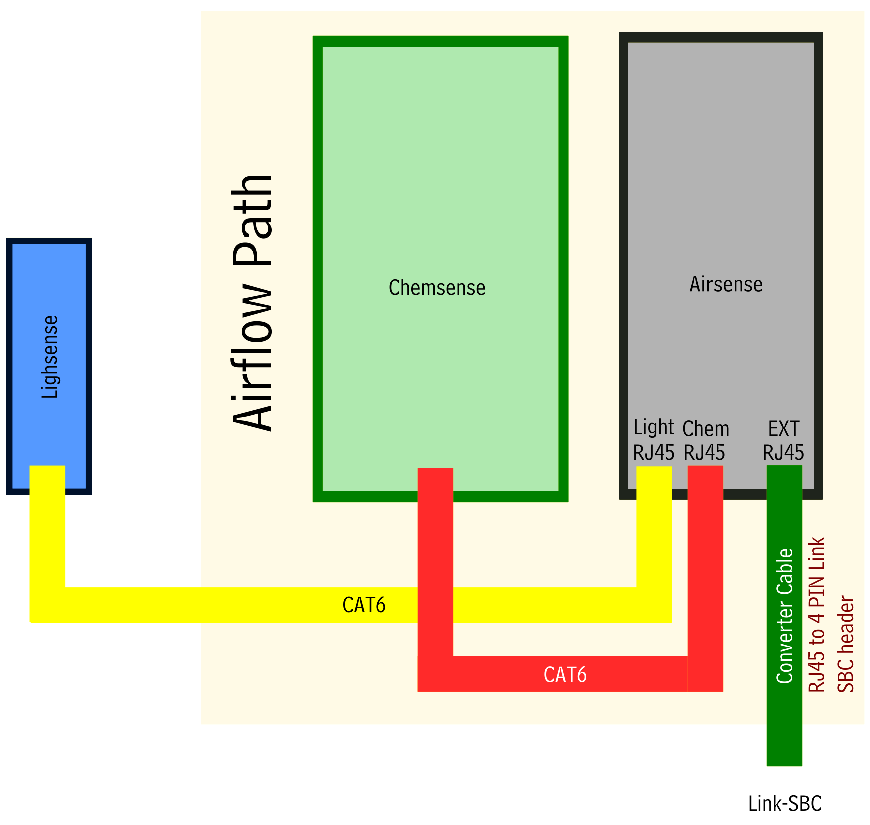
\includegraphics[width=4in]{link.pdf}
\caption{Connections between the sensor boards and interface to Link SBC}
\label{fig:physicalConnections}
\end{center}
\end{figure}


\section{Data Transmission} \label{section:overall}

The data from the sensor boards is sent as a formatted unit of data -- a transmission
packet. A transmission packet is composed of several data sub-packets, each
of which carries information pertaining to the parameter listed in the sub-packet.
The data sub-packet, especially for additional sensors, rain gauge and soil moisture sensor, are described here.

\subsection{Data Sub-packets} \label{ssec:sub-pack}

The data segment of the transmission packet is further broken down into many
sub-packets. The sub-packet starts with a source identifier. One bit
validity field and seven bits ``length of the sub-packet'' field
are packed together as the next byte. The length field counts the number of
bytes following it which make up the sub-packet. The table below shows the organization
of a rain gauge sub-packet. 
\par
If the field is set to 1, it indicates a valid measurement/reading, 
and if the validity bit is set to 0 if the sensor represented in the sub-packet
is dead, disabled, unconnected, unresponsive or if data could not be collected
from the sensor in the time window. If the validity is 0, the particular invalid sub-packet is not packed into a transmission packet.

\subsubsection{Rain Gauge}
As shown in Table \ref{table:rain_subpacket}, sensor identifier of rain gauge is 0xFC, which is 252 in decimal, and if the data are valid, second byte will be 0x84, which means the sub-packet is valid and length of the sub-packet is 4 Bytes.


\begin{table}[H]
    \centering {
    \begin{tabular}{|c|c|c|c|}
        \hline
        \rowcolor{black!8}
        \textbf{Source ID} & \bf{1-bit Validity [0: invalid, 1: valid] | 7-bit Data Length} & \textbf{Data} \\
        \rowcolor{black!8}
        (1 Byte) & (1 Byte) & (2 Bytes) \\
        \hline
        0xFC & 0x84 (valid) & count of pendant event\\ 
        \hline
    \end{tabular}
    }
    \caption{Sub-packet for rain gauge}
    \label{table:rain_subpacket}
\end{table}


\subsubsection{Soil Moisture Sensor}
As shown in Table \ref{table:soil_subpacket}, sensor identifier of soil sensor is 0xFB, which is 251 in decimal,
and if the data are valid, second byte will be 0x84, which means the sub-packet is valid and length of the sub-packet is
6 Bytes.


\begin{table}[H]
    \centering {
    \begin{tabular}{|c|c|c|c|c|}
        \hline
        \rowcolor{black!8}
        \textbf{Source ID} & \bf{1-bit Validity | 7-bit Data Length} & \textbf{Data} \\
        \rowcolor{black!8}
        (1 Byte) & [0: invalid, 1: valid]  (1 Byte) & (6 Bytes) \\
        \hline
        \multirow{3}{*}{0xFB} & \multirow{3}{*}{0x86 (valid)} & Dielectric permittivity in Format 6 (2 Bytes) \\ \cline{3-3}
        & & Electric Conductivity in Format 6 (2 Bytes) \\ \cline{3-3}
        & & Temperature in Format 6 (2 Bytes) \\ \hline
    \end{tabular}
    }
    \caption{Sub-packet for rain gauge}
    \label{table:soil_subpacket}
\end{table}


\subsection{Data Formats}

The data sent in each sub-packet is encoded in one or more formats. Currently we define eight formats for various types of data including integers, bytes, and floating point numbers. 
Rain gauge data encoded as format 1, which is integers in range 0 to 65535, as shown in Table \ref{table:rain_format}.
Therefore the data of the rain gauge is an integer, and it means the count of pendant event inside the rain gauge. One event of the pendant means 0.01 in. (0.254 mm) of precipitation.
Soil sensor data is encoded as format 6, which is integers in range $-$127.99 to 127.99, as shown in Table \ref{table:rain_format}.
Therefore the data of the soil sensor are float point dielectric, conductivity, and temperature.
\\


\begin{table}[H]
    \centering {
    \begin{tabular}{|c|c|c|c|}
        \hline
        \rowcolor{black!8}
        \textbf{Format} & \textbf{Number of Bytes Used} & \textbf{Value Represented} & \textbf{Value Range} \\
        \hline
        1 & 2 & unsigned int\_16 input & 0 -- 65535 \\ %& MSByte LSByte\\
        6 & 2 & float input & [$-$127.99, 127.99] \\
        \hline
    \end{tabular}
    }
    \caption{Data format for rain gauge}
    \label{table:rain_format}
\end{table}

\clearpage
\section{Data Sub-Packet} \label{section:dataSub}

The data sub-packet consists of 32 "chunks" (30 sensors and 2 MAC addresses).  Each "chunk" follows one of seven formats.\\

%%%%%%%%%%%%%%%%%%%%

\subsection{Data Formats}

\begin{table}[H]
    \centering
    {\rowcolors{2}{black!12}{black!2}
    \begin{tabular}{|c c c c c c c|}
        \hline
        \textbf{Format} & \textbf{Byte 0} & \textbf{Byte 1} & \textbf{Byte 2} & \textbf{Byte 3} & \textbf{Byte 4} & \textbf{Byte 5}\\
        \hline
        \hline
        1 & (1 << 7) | 7-bit int & (neg << 7) | 7-bit frac. & - & - & - & -\\
        2 & 7 MSb & LSB & - & - & - & -\\
        3 & Addr5 & Addr4 & Addr3 & Addr2 & Addr1 & Addr0\\
        4 &
        \multirow{1}{8em}{(1 << 7) | (neg << 6) | (4-bit int << 2) | 2 MSb of frac.}
        & 8 LSb of frac. & - & - & - & -\\[4ex]
        5 & (neg << 6) | 6 MSb & 8 LSb & - & - & - & -\\
        6 &
        \multirow{1}{9em}{(1 << 7) | (neg << 6) | 6 MSb}
        & Middle 8 bits & 8 LSb & - & - & -\\[2ex]
        7 & First 8 "chunks" & 8 "chunks" & 8 "chunks" & Last 8 "chunks" & - & -\\
        \hline
    \end{tabular}
    }
    \caption{Data formats}
    \label{table:overall}
\end{table}

This version of the Waggle protocol does not use standard representations for floating point numbers.  Instead, the location of the decimal point is pre-determined (between the integer and fractional components, if applicable).\\

The most significant bit in byte 0 of formats 1, 4, and 6 means the data is already converted.  Formats 2 and 5 contain raw data.\\

Formats 1, 4, 5, and 6 contain a "negative" bit.  If this bit is 1, the value is negative.

%%%%%%%%%%%%%%%%%%%%

\subsection{Data "Chunks"}

The \textit{length} in each data "chunk" represents the number of bytes of sensor data.  The total "chunk" length is \textit{length} + 2.

\begin{table}[H]
    \centering
    {\rowcolors{2}{black!15}{black!8}
    \begin{tabular}{|c c c c|}
        \hline
        \textbf{Field} & \textbf{ID} & \textbf{Validity | Length} & \textbf{Data}\\
        \hline
        \hline
        Main MAC address & 0x00 & (1 << 7) | 0x06 & Table \ref{table:sensor1}\\
        TMP112 & 0x01 & (0/1 << 7) | 0x02 & Table \ref{table:sensor2}\\
        HTU21D & 0x02 & (0/1 << 7) | 0x04 & Table \ref{table:sensor3}\\
        GP2Y1010AU0F & 0x03 & (0/1 << 7) | 0x02 & Table \ref{table:sensor4}\\
        BMP180 & 0x04 & (0/1 << 7) | 0x05 & Table \ref{table:sensor5}\\
        PR103J2 & 0x05 & (0/1 << 7) | 0x02 & Table \ref{table:sensor6}\\
        TSL250RD & 0x06 & (0/1 << 7) | 0x02 & Table \ref{table:sensor6}\\
        MMA8452Q & 0x07 & (0/1 << 7) | 0x08 & Table \ref{table:sensor7}\\
        SPV1840LR5H-B & 0x08 & (0/1 << 7) | 0x02 & Table \ref{table:sensor8}\\
        TSYS01 & 0x09 & (0/1 << 7) | 0x02 & Table \ref{table:sensor9}\\
        HMC5883L & 0x0A & (0/1 << 7) | 0x06 & Table \ref{table:sensor10}\\
        HIH6130 & 0x0B & (0/1 << 7) | 0x04 & Table \ref{table:sensor3}\\
        APDS-9006-020 & 0x0C & (0/1 << 7) | 0x02 & Table \ref{table:sensor6}\\
        TSL260RD & 0x0D & (0/1 << 7) | 0x02 & Table \ref{table:sensor6}\\
        TSL250RD & 0x0E & (0/1 << 7) | 0x02 & Table \ref{table:sensor6}\\
        MLX75305 & 0x0F & (0/1 << 7) | 0x02 & Table \ref{table:sensor6}\\
        ML8511 & 0x10 & (0/1 << 7) | 0x02 & Table \ref{table:sensor6}\\
        D6T & 0x11 & (0/1 << 7) | 0x22 & Table \ref{table:sensor11}\\
        MLX90614 & 0x12 & (0/1 << 7) | 0x02 & Table \ref{table:sensor2}\\
        TMP421 & 0x13 & (0/1 << 7) | 0x02 & Table \ref{table:sensor2}\\
        SPV1840LR5H-B & 0x14 & (0/1 << 7) | 0x02 & Table \ref{table:sensor8}\\
        Total reducing gases & 0x15 & (0/1 << 7) | 0x02 & Table \ref{table:sensor12}\\
        Ethanol & 0x16 & (0/1 << 7) | 0x02 & Table \ref{table:sensor12}\\
        Nitrogen dioxide & 0x17 & (0/1 << 7) | 0x02 & Table \ref{table:sensor12}\\
        Ozone & 0x18 & (0/1 << 7) | 0x02 & Table \ref{table:sensor12}\\
        Hydrogen sulphide & 0x19 & (0/1 << 7) | 0x02 & Table \ref{table:sensor12}\\
        Total oxidizing gases & 0x1A & (0/1 << 7) | 0x02 & Table \ref{table:sensor12}\\
        Carbon monoxide & 0x1B & (0/1 << 7) | 0x02 & Table \ref{table:sensor12}\\
        Sulfur dioxide & 0x1C & (0/1 << 7) | 0x02 & Table \ref{table:sensor12}\\
        Sensirion & 0x1D & (0/1 << 7) | 0x04 & Table \ref{table:sensor3}\\
        Bosh & 0x1E & (0/1 << 7) | 0x03 & Table \ref{table:sensor13}\\
        Intel MAC address & 0x1F & (1 << 7) | 0x06 & Table \ref{table:sensor1}\\
        Sensor status (health) & 0xFE & (1 << 7) | 0x04 & Table \ref{table:sensor14}\\
        \hline
    \end{tabular}
    }
    \caption{Data sub-packet structure (each row is a "chunk")}
    \label{table:dataChunk}
\end{table}

\begin{table}[H]
    \centering
    {\rowcolors{2}{black!12}{black!2}
    \begin{tabular}{|c c c c c c|}
        \hline
        \textbf{Byte 0} & \textbf{Byte 1} & \textbf{Byte 2} & \textbf{Byte 3} & \textbf{Byte 4} & \textbf{Byte 5}\\
        \hline
        \hline
        Address 5 & Address 4 & Address 3 & Address 2 & Address 1 & Address 0\\
        \multicolumn{6}{|c|}{Format 3}\\
        \hline
    \end{tabular}
    }
    \caption{MAC address}
    \label{table:sensor1}
\end{table}

\begin{table}[H]
    \centering
    {\rowcolors{2}{black!12}{black!2}
    \begin{tabular}{|c c|}
        \hline
        \textbf{Byte 0} & \textbf{Byte 1}\\
        \hline
        \hline
        \multicolumn{2}{|c|}{Temperature}\\
        \multicolumn{2}{|c|}{Format 1}\\
        \hline
    \end{tabular}
    }
    \caption{Sensor data}
    \label{table:sensor2}
\end{table}

\begin{table}[H]
    \centering
    {\rowcolors{2}{black!12}{black!2}
    \begin{tabular}{|c c c c|}
        \hline
        \textbf{Byte 0} & \textbf{Byte 1} & \textbf{Byte 2} & \textbf{Byte 3}\\
        \hline
        \hline
        \multicolumn{2}{|c|}{Temperature} & \multicolumn{2}{|c|}{Humidity}\\
        \multicolumn{2}{|c|}{Format 1} & \multicolumn{2}{|c|}{Format 1}\\
        \hline
    \end{tabular}
    }
    \caption{Sensor data}
    \label{table:sensor3}
\end{table}

\begin{table}[H]
    \centering
    {\rowcolors{2}{black!12}{black!2}
    \begin{tabular}{|c c|}
        \hline
        \textbf{Byte 0} & \textbf{Byte 1}\\
        \hline
        \hline
        \multicolumn{2}{|c|}{Dust}\\
        \multicolumn{2}{|c|}{Format 2}\\
        \hline
    \end{tabular}
    }
    \caption{Sensor data}
    \label{table:sensor4}
\end{table}

\begin{table}[H]
    \centering
    {\rowcolors{2}{black!12}{black!2}
    \begin{tabular}{|c c c c c|}
        \hline
        \textbf{Byte 0} & \textbf{Byte 1} & \textbf{Byte 2} & \textbf{Byte 3} & \textbf{Byte 4}\\
        \hline
        \hline
        \multicolumn{2}{|c|}{Temperature} & \multicolumn{3}{|c|}{Atmospheric pressure}\\
        \multicolumn{2}{|c|}{Format 1} & \multicolumn{3}{|c|}{Format 6}\\
        \hline
    \end{tabular}
    }
    \caption{Sensor data}
    \label{table:sensor5}
\end{table}

\begin{table}[H]
    \centering
    {\rowcolors{2}{black!12}{black!2}
    \begin{tabular}{|c c|}
        \hline
        \textbf{Byte 0} & \textbf{Byte 1}\\
        \hline
        \hline
        \multicolumn{2}{|c|}{Light}\\
        \multicolumn{2}{|c|}{Format 2}\\
        \hline
    \end{tabular}
    }
    \caption{Sensor data}
    \label{table:sensor6}
\end{table}

\begin{table}[H]
    \centering
    {\rowcolors{2}{black!12}{black!2}
    \begin{tabular}{|c c c c c c c c|}
        \hline
        \textbf{Byte 0} & \textbf{Byte 1}  & \textbf{Byte 2} & \textbf{Byte 3} & \textbf{Byte 4} & \textbf{Byte 5} & \textbf{Byte 6} & \textbf{Byte 7}\\
        \hline
        \hline
        \multicolumn{2}{|c|}{Acceleration X} & \multicolumn{2}{|c|}{Acceleration Y}  & \multicolumn{2}{|c|}{Acceleration Z} & \multicolumn{2}{|c|}{RMS}\\
        \multicolumn{2}{|c|}{Format 1} & \multicolumn{2}{|c|}{Format 1}  & \multicolumn{2}{|c|}{Format 1} & \multicolumn{2}{|c|}{Format 1}\\
        \hline
    \end{tabular}
    }
    \caption{Sensor data}
    \label{table:sensor7}
\end{table}

\begin{table}[H]
    \centering
    {\rowcolors{2}{black!12}{black!2}
    \begin{tabular}{|c c|}
        \hline
        \textbf{Byte 0} & \textbf{Byte 1}\\
        \hline
        \hline
        \multicolumn{2}{|c|}{Sound pressure}\\
        \multicolumn{2}{|c|}{Format 2}\\
        \hline
    \end{tabular}
    }
    \caption{Sensor data}
    \label{table:sensor8}
\end{table}

\begin{table}[H]
    \centering
    {\rowcolors{2}{black!12}{black!2}
    \begin{tabular}{|c c|}
        \hline
        \textbf{Byte 0} & \textbf{Byte 1}\\
        \hline
        \hline
        \multicolumn{2}{|c|}{Temperature}\\
        \multicolumn{2}{|c|}{Format 2}\\
        \hline
    \end{tabular}
    }
    \caption{Sensor data}
    \label{table:sensor9}
\end{table}

\begin{table}[H]
    \centering
    {\rowcolors{2}{black!12}{black!2}
    \begin{tabular}{|c c c c c c|}
        \hline
        \textbf{Byte 0} & \textbf{Byte 1}  & \textbf{Byte 2} & \textbf{Byte 3} & \textbf{Byte 4} & \textbf{Byte 5}\\
        \hline
        \hline
        \multicolumn{2}{|c|}{Magnetic X} & \multicolumn{2}{|c|}{Magnetic Y}  & \multicolumn{2}{|c|}{Magnetic Z}\\
        \multicolumn{2}{|c|}{Format 4} & \multicolumn{2}{|c|}{Format 4}  & \multicolumn{2}{|c|}{Format 4}\\
        \hline
    \end{tabular}
    }
    \caption{Sensor data}
    \label{table:sensor10}
\end{table}

\begin{table}[H]
    \centering
    {\rowcolors{2}{black!12}{black!2}
    \begin{tabular}{|c c c c c|}
        \hline
        \textbf{Byte 0} & \textbf{Byte 1} & \textbf{...} & \textbf{Byte 32} & \textbf{Byte 33}\\
        \hline
        \hline
        \multicolumn{2}{|c|}{Temperature} & Temperature & \multicolumn{2}{|c|}{Temperature}\\
        \multicolumn{2}{|c|}{Format 1} & Format 1 & \multicolumn{2}{|c|}{Format 1}\\
        \hline
    \end{tabular}
    }
    \caption{Sensor data}
    \label{table:sensor11}
\end{table}

\begin{table}[H]
    \centering
    {\rowcolors{2}{black!12}{black!2}
    \begin{tabular}{|c c|}
        \hline
        \textbf{Byte 0} & \textbf{Byte 1}\\
        \hline
        \hline
        \multicolumn{2}{|c|}{Gas concentration}\\
        \multicolumn{2}{|c|}{Format 2}\\
        \hline
    \end{tabular}
    }
    \caption{Sensor data}
    \label{table:sensor12}
\end{table}

\begin{table}[H]
    \centering
    {\rowcolors{2}{black!12}{black!2}
    \begin{tabular}{|c c c|}
        \hline
        \textbf{Byte 0} & \textbf{Byte 1} & \textbf{Byte 2}\\
        \hline
        \hline
        \multicolumn{3}{|c|}{Atmospheric pressure}\\
        \multicolumn{3}{|c|}{Format 6}\\
        \hline
    \end{tabular}
    }
    \caption{Sensor data}
    \label{table:sensor13}
\end{table}

\begin{table}[H]
    \centering
    {\rowcolors{2}{black!12}{black!2}
    \begin{tabular}{|c c c c|}
        \hline
        \textbf{Byte 0} & \textbf{Byte 1} & \textbf{Byte 2}  & \textbf{Byte 3}\\
        \hline
        \hline
        \multicolumn{4}{|c|}{Health status (1 bit per "chunk")}\\
        \multicolumn{4}{|c|}{Format 7}\\
        \hline
    \end{tabular}
    }
    \caption{Sensor status (health)}
    \label{table:sensor14}
\end{table}

%%%%%%%%%%%%%%%%%%%%
\newpage
\section{Sub-packets}

As shortly explained in document section \ref{ssec:sub-pack}, data sub-packets are generated depending on its designated data format and length when data reading from each sensor if valid. The first byte of the sub-packet is sensor ID for each parameter, and the second byte means validity of the packet and length of the sensor data as shown in Table \ref{table:packsegments}. Detail of sub-packet and sensor data will be explined in this section.


\subsection{Parameters}

The sensor boards output a set of parameters which are identified by a unique ID. Each parameter
has a set of values associated with it which are encoded in an appropriate data format. The table
below lists the various parameters produced by the sensor boards, the unique source ID used to identify them, the values produced by them and the format in which the value is encoded.
\par
Each parameter and its values are composed into a sub-packet based on
the format described in document section \ref{ssec:sub-pack}.
In the case of parameters with 2 or more values, the encoded values are
arranged in the sub-packets sequentially. 


\begin{center}
\begin{longtable}{|l|c|>{\centering}p{0.3\textwidth}|c|}
\caption{Data sub-packet structure (each row is a "chunk")} \label{tab:dataChunk} \\

\hline \rowcolor{black!8} \multicolumn{1}{|c|}{\textbf{Parameter}} & \multicolumn{1}{c|}{\textbf{Source ID}} & \multicolumn{1}{c|}{\textbf{Values}} & \multicolumn{1}{c|}{\textbf{Formats}} \\ \hline
\endfirsthead

\multicolumn{4}{c}%
{{\bfseries \tablename \thetable{} -- continued from previous page}} \\
\hline \rowcolor{black!8} \multicolumn{1}{|c|}{\textbf{Parameter}} & \multicolumn{1}{c|}{\textbf{Source ID}} & \multicolumn{1}{c|}{\textbf{Values}} & \multicolumn{1}{c|}{\textbf{Formats}} \\ \hline 
\endhead

% \rowcolor{black!8} \multicolumn{4}{|r|}{{Continued on next page}} \\ \hline
\endfoot

\hline
\endlastfoot

        \multirow{3}{*}{Firmware version} & \multirow{3}{*}{0xFD} & Firmware version (HW/SW) & \multirow{3}{*}{Bit mask} \\ \cline{3-3}
        & & Build time & \\ \cline {3-3} 
        & & Build git & \\ \hline

    \rowcolor{black!5} \multicolumn{4}{|c|}{{Airsense board}} \\ \hline
        Airsense/Lightsense MAC address & 0x00 & MAC Address & Format 3 \\ \hline
        TMP112 & 0x01 & Temperature & Format 6\\ \hline
        \multirow{2}{*}{HTU21D} & \multirow{2}{*}{0x02} & Temperature & \multirow{2}{*}{Format 6}\\ \cline{3-3}
        & & relative humidity & \\ \hline
        \multirow{2}{*}{BMP180} & \multirow{2}{*}{0x04} & Temperature & Format 6\\ \cline{3-4}
        & & Pressure & Format 4 \\ \hline
        PR103J2 & 0x05 & Temperature & Format 1\\ \hline
        TSL250RD & 0x06 & Visible Light & Format 1\\ \hline
        \multirow{4}{*}{MMA8452Q} & \multirow{4}{*}{0x07} & Acceleration in X & \multirow{4}{*}{Format 6}\\ \cline{3-3}
        & & Acceleration in Y & \\ \cline{3-3}
        & & Acceleration in Z & \\ \cline{3-3}
        & & Vibration & \\ \hline
        SPV1840LR5H-B & 0x08 & RMS Sound Level & Format 1\\ \hline
        TSYS01 & 0x09 & Temperature & Format 6\\ \hline
        
    \rowcolor{black!8} \multicolumn{4}{|c|}{{Lightsense board}} \\ \hline
        \multirow{3}{*}{HMC5883L} & \multirow{3}{*}{0x0A} & Magnetic Field in Z & \multirow{3}{*}{Format 8}\\ \cline{3-3}
        & & Magnetic Field in Y & \\ \cline{3-3}
        & & Magnetic Field in Z & \\ \hline
        \multirow{2}{*}{HIH6130} & \multirow{2}{*}{0x0B} & Temperature & \multirow{2}{*}{Format 6}\\ \cline{3-3}
        & & relative humidity & \\ \hline
        APDS-9006-020 & 0x0C & Ambient light intensity & Format 1\\ \hline
        TSL260RD & 0x0D & IR intensity & Format 1\\ \hline
        TSL250RD & 0x0E & Visible light intensity & Format 1\\ \hline
        MLX75305 & 0x0F & Light & Format 1\\ \hline 
        ML8511 & 0x10 & UV intensity & Format 1\\ \hline
        TMP421 & 0x13 & Temperature & Format 6\\ \hline
        SPV1840LR5H-B & 0x14 & RMS Sound Level & Format 1\\ \hline

    \rowcolor{black!8} \multicolumn{4}{|c|}{{Chemsense board}} \\ \hline
        Total reducing gases & 0x15 & \multirow{7}{*}{Raw Concentration} & \multirow{7}{*}{Format 5}\\ \cline{1-2}
        Nitrogen dioxide & 0x17 & & \\ \cline{1-2}
        Ozone & 0x18 & & \\ \cline{1-2}
        Hydrogen sulphide & 0x19 & &\\ \cline{1-2}
        Total oxidizing gases & 0x1A & &\\ \cline{1-2}
        Carbon monoxide & 0x1B & &\\ \cline{1-2}
        Sulfur dioxide & 0x1C & &\\ \hline
        \multirow{2}{*}{SHT25} & \multirow{2}{*}{0x1D} & Temperature & \multirow{2}{*}{Format 2}\\ \cline{3-3}
        & & relative humidity & \\ \hline
        \multirow{2}{*}{LPS25H} & \multirow{2}{*}{0x1E} & Temperature & Format 2\\ \cline{3-4}
        & & Pressure & Format 4\\ \hline
        \multirow{3}{*}{Si1145} & \multirow{3}{*}{0x1F} & UV intensity & \multirow{3}{*}{Format 1} \\ \cline{3-3}
        & & Visible light intensity & \\ \cline{3-3}
        & & IR intensity & \\ \hline
        Chemsense MAC address & 0x20 & MAC Address & Format 3\\ \hline
        CO ADC temp & 0x21 & \multirow{2}{*}{ADC temperature} &  \multirow{2}{*}{Format 2}\\ \cline{1-2}
        IAQ IRR ADC temp & 0x22 & &\\ \hline
        O3 NO2 ADC temp & 0x23 & \multirow{3}{*}{ADC temperature} &  \multirow{3}{*}{Format 2} \\ \cline{1-2}
        SO2 H2S ADC temp & 0x24 & & \\ \cline{1-2}
        CO LMP temp & 0x25 & &\\ \hline
        \multirow{4}{*}{Accelerometer} & \multirow{4}{*}{0x26} & Acceleration in X & \multirow{3}{*}{Format 2} \\ \cline{3-3}
        & & Acceleration in Y & \\ \cline{3-3}
        & & Acceleration in Z & \\ \cline{3-4}
        & & Vibration & Format 4\\ \hline
        \multirow{4}{*}{Gyro} & \multirow{4}{*}{0x27} & Orientation in X & \multirow{3}{*}{Format 2} \\ \cline{3-3}
        & & Orientation in Y & \\ \cline{3-3}
        & & Orientation in Z & \\ \cline {3-4}
        & & Orientation Index & Format 4\\ \hline

     \rowcolor{black!8} \multicolumn{4}{|c|}{{Alpha Sensor}} \\ \hline
        \multirow{9}{*}{Histogram} & \multirow{9}{*}{0x28} & Bin count & \multirow{20}{*}{Raw reading} \\ \cline{3-3}
        & & Average Time &\\ \cline{3-3}
        & & Sample flow rate &\\ \cline{3-3}
        & & Temp/Pressure(alther) &\\ \cline{3-3}
        & & Sampling period &\\ \cline{3-3}
        & & Sum of the counts &\\ \cline{3-3}
        & & PM 1 &\\ \cline{3-3}
        & & PM 2.5 &\\ \cline{3-3}
        & & PM 10 &\\ \cline{1-3}
        Firmware & 0x29 & Firmware version & \\ \cline{1-3}
        \multirow{2}{*}{Configuration A} & \multirow{2}{*}{0x30} & Bin Boundaries &\\ \cline{3-3}
        & & Bin Particle Volumes A &\\ \cline{1-3}
        \multirow{2}{*}{Configuration B} & \multirow{2}{*}{0x31} & Bin Particle Volumes B &\\ \cline{3-3}
        & & Bin Particle Densities A &\\ \cline{1-3}
        \multirow{2}{*}{Configuration C} & \multirow{2}{*}{0x32} & Bin Particle Densities B &\\ \cline{3-3}
        & & Bin Sample Volume Weightings A &\\ \cline{1-3}
        \multirow{6}{*}{Configuration D} & \multirow{6}{*}{0x33} & Bin Sample Volume Weightings B &\\ \cline{3-3}
        & & Gain Scaling Coefficient & \\ \cline{3-3}
        & & Sample Flow Rate & \\ \cline{3-3}
        & & Laser DAC and Fan DAC & \\ \cline{3-3}
        & & Conversion factor & \\ \cline{3-3}
        & & Space Bytes & \\ 

\end{longtable}
\end{center}


\subsection{Data packets}
The context of each parameter, its utility and the arrangement of its values is described below. In all
the tables below, the validity bit is set to 1, which means the data is valid. The parameter descriptions
below are aggregated based on the sensor-board they are situated on -
Metsense, Lightsense and Chemsense.

\subsubsection{Firmware Version}
This is a 8 bytes version information that identifies hardware version, software version, and build information of the waggle node.
The build time and the build git are included to varify the effectiveness of the software.
Firmware version is bit masked and encoded through format 1, and build git is encoded through format 1.

\begin{table}[h!]
    \centering
    \caption{Sub-packet of Firmware version}
    \begin{tabular}{|c|c|c|c|c|}
        \hline
        \rowcolor{black!8}
        \textbf{0xFD} & \textbf{0x88} & \textbf{Firmware version in Format 1} & \textbf{Build time} & \textbf{Build git in Format 1} \\ \hline
        Byte[0] & Byte[1] & Bytes[2 -- 3] & Bytes[4 -- 7] & Bytes[8 -- 9]\\ \hline
    \end{tabular}
\end{table}


\newcolumntype{a}{>{\columncolor{black!8}}c}
\begin{table}[h!]
    \centering
    \caption{Firmware version}
    \begin{tabular}{|a|c|}
        \hline
        \textbf{3 bit major HW ver. | 3 bit minor HW ver. | 2 bit major SW ver.} & Byte[2] \\ \hline
        \textbf{2 bit major SW ver. | minor SW ver. $\times$ 10 + sub SW ver.} & Byte[3]\\ \hline
    \end{tabular}
\end{table}

\end{document}
